%% main.tex — Projeto de Pesquisa
%% FFCLRP-USP — Programa de Pós-Graduação em Computação Aplicada
%% Autor: Cássio Silva Takarada
%% Orientador: Prof. Dr. Luiz Otávio Murta Junior
%%
%% Estrutura em três pilares (Proposta, Conteúdo Teórico, Estado da Arte),
%% conforme a fase F7 do plano de trabalho.

\documentclass[
  12pt,
  openright,
  oneside,
  a4paper,
  english,
  brazil,
]{abntex2}

%% ─── Pacotes ────────────────────────────────────────────────────────────────
\usepackage[T1]{fontenc}
\usepackage[utf8]{inputenc}
\usepackage{lmodern}
\usepackage{microtype}
\usepackage{indentfirst}
\usepackage{amsmath,amssymb}
\usepackage{graphicx}
\usepackage{float}
\usepackage{booktabs}
\usepackage{multirow}
\usepackage{siunitx}
\usepackage{hyperref}
\usepackage[alf,abnt-emphasize=bf]{abntex2cite}

\sisetup{output-decimal-marker={,}, group-separator={.}, group-digits=integer}

%% ─── Metadados ──────────────────────────────────────────────────────────────
\titulo{Complexidade estatística dos pesos como indicador de overfitting
independente do conjunto de validação}
\autor{Cássio Silva Takarada}
\local{Ribeirão Preto}
\data{2026}
\orientador{Prof. Dr. Luiz Otávio Murta Junior}
\instituicao{Universidade de São Paulo \\
Faculdade de Filosofia, Ciências e Letras de Ribeirão Preto \\
Departamento de Computação e Matemática}
\tipotrabalho{Projeto de Pesquisa}

\preambulo{Projeto de pesquisa apresentado ao Programa de Pós-Graduação em
Computação Aplicada da Faculdade de Filosofia, Ciências e Letras de Ribeirão
Preto da Universidade de São Paulo.}

\hyphenation{over-fitting under-fitting gro-kking}

\begin{document}

\selectlanguage{brazil}
\frenchspacing

\imprimircapa
\imprimirfolhaderosto

\begin{resumo}
O diagnóstico de \emph{overfitting} em redes neurais profundas depende hoje,
integralmente, de um conjunto de validação rotulado, representativo e
suficientemente grande --- condição frequentemente inviável em imagens médicas,
onde a anotação é cara e exige especialista. Este projeto investiga se medidas
de complexidade estatística calculadas \emph{exclusivamente sobre os pesos} da
camada densa de uma rede, sem acesso a rótulo algum, fornecem ao desenvolvedor
uma leitura do estado do treinamento independente da validação. São
consideradas a complexidade LMC, a entropia amostral unidimensional (SampEn) e
a entropia amostral bidimensional (SampEn2D), acompanhadas ao longo das épocas
de treino. Resultados preliminares com a rede ResNet-18 sobre o repositório
MedNIST, em oito pares de execuções com e sem corrupção controlada de rótulos,
indicam que a SampEn2D da camada densa inflete, em média,
\num{7,5} $\pm$ \num{0,9} épocas antes da degradação da acurácia de validação,
com razão de amplitude de \num{5,7} vezes entre execuções com e sem
memorização ($p = \num{0,00016}$), enquanto a complexidade LMC não discrimina
as duas condições ($p = \num{0,33}$). Pretende-se consolidar esses achados,
caracterizar os limites de generalização entre arquiteturas e entregar um
monitor acoplável a qualquer laço de treinamento em PyTorch.
\textbf{Palavras-chave}: complexidade estatística; entropia amostral;
\emph{overfitting}; aprendizado profundo; imagens médicas.
\end{resumo}

\tableofcontents

\textual
\chapter{Proposta}
\label{cap:proposta}

\section{Contextualização e Motivação}
\label{sec:P-contexto}

O aprendizado profundo consolidou-se como abordagem dominante em tarefas de
classificação e segmentação de imagens médicas. Esse sucesso, contudo, apoia-se
em uma premissa que a prática clínica raramente satisfaz: a disponibilidade de
grandes conjuntos de dados anotados. Em imagens médicas, a anotação exige um
especialista, é onerosa e lenta, e frequentemente esbarra em restrições éticas
e de privacidade que limitam o compartilhamento entre instituições.

Essa escassez tem uma consequência metodológica pouco discutida. O procedimento
padrão para decidir quando interromper o treinamento --- o \emph{early
stopping} --- monitora o erro em um conjunto de validação separado e interrompe
o ajuste quando esse erro deixa de diminuir \cite{prechelt1998}. O
procedimento é sólido, mas transfere para o conjunto de validação toda a
responsabilidade pelo diagnóstico: se ele é pequeno, desbalanceado ou pouco
representativo, a estimativa do momento de parada torna-se ruidosa, e o
desenvolvedor não dispõe de nenhum sinal alternativo para confrontá-la. Em
outras palavras, justamente no regime de poucos dados --- aquele em que o
\emph{overfitting} é mais provável --- o instrumento de medida é o menos
confiável.

Há, entretanto, uma fonte de informação sobre o estado do treinamento que
permanece pouco explorada e que não depende de rótulo algum: os próprios pesos
da rede. A memorização de exemplos deixa marcas na distribuição de valores dos
parâmetros, e trabalhos consolidados mostram que redes profundas são capazes de
ajustar rótulos completamente aleatórios \cite{zhang2017}, memorizando-os por um
regime de aprendizado distinto daquele em que extraem padrões
generalizáveis \cite{arpit2017}. Se esses dois regimes deixam assinaturas
distinguíveis na estrutura dos pesos, então medidas de complexidade estatística
aplicadas a esses pesos podem, em princípio, sinalizar a transição entre eles
sem consultar nenhum dado rotulado.

\section{Problema de Pesquisa}
\label{sec:P-problema}

É possível detectar o início do \emph{overfitting} de uma rede neural profunda
a partir exclusivamente da complexidade estatística de seus pesos, sem recorrer
a um conjunto de validação rotulado?

\section{Hipótese}
\label{sec:P-hipotese}

A hipótese central deste trabalho é a de que a transição do regime de
aprendizado generalizante para o regime de memorização produz uma mudança
mensurável na irregularidade estrutural dos pesos da camada densa, e que essa
mudança \emph{antecede} a degradação observável no conjunto de validação.

Operacionalmente, espera-se que, em execuções nas quais o \emph{overfitting} é
induzido de forma controlada, ao menos um dos indicadores considerados apresente
inflexão em uma época anterior àquela em que a acurácia de validação começa a
cair de modo sustentado, e que essa inflexão não ocorra --- ou ocorra de forma
substancialmente atenuada --- em execuções de controle sem indução. A hipótese
é falsificável: caso a inflexão ocorra simultaneamente ou posteriormente à
degradação da validação, ou caso ocorra com a mesma intensidade nas execuções
de controle, o indicador não tem valor como aviso antecipado e isso deve ser
reportado como tal.

\section{Objetivos}
\label{sec:P-objetivos}

\subsection{Objetivo Geral}

Avaliar a complexidade estatística dos pesos de redes neurais profundas como
indicador de \emph{overfitting} independente do conjunto de validação,
entregando ao desenvolvedor um instrumento de diagnóstico acoplável ao laço de
treinamento.

\subsection{Objetivos Específicos}

\begin{enumerate}
    \item Implementar, em um módulo único e validado numericamente, a
          complexidade LMC, a entropia amostral unidimensional (SampEn) e a
          entropia amostral bidimensional (SampEn2D), estabelecendo-o como
          fonte única de cálculo para todo o trabalho.
    \item Formalizar a leitura dos pesos da camada densa como objeto de
          medida, fixando a ordem de achatamento da matriz de pesos e
          justificando-a experimentalmente.
    \item Definir operacionalmente o início do \emph{overfitting} e construir
          um protocolo de indução controlada por corrupção de rótulos, com
          execuções de controle pareadas.
    \item Implementar um monitor que calcule os indicadores a cada época
          durante o treinamento e emita um estado do aprendizado em tempo real.
    \item Quantificar a antecedência de cada indicador em relação à degradação
          da validação, com múltiplas sementes e teste de significância.
    \item Caracterizar os limites do indicador quanto ao nível de corrupção e
          quanto à arquitetura da rede, reportando explicitamente os regimes em
          que ele falha.
\end{enumerate}

\section{Justificativa: o ponto de vista do desenvolvedor}
\label{sec:P-justificativa}

A justificativa deste trabalho é deliberadamente formulada do ponto de vista de
quem treina a rede, e não apenas do ponto de vista teórico.

\subsection{A dependência atual dos dados rotulados}

Para saber se uma rede aprendeu ou apenas memorizou, o desenvolvedor depende
hoje inteiramente dos dados. É preciso construir conjuntos de treino, validação
e teste que sejam bem particionados, corretamente rotulados e representativos da
população de interesse. Cada um desses requisitos custa tempo e dinheiro, e em
imagens médicas frequentemente esbarra na indisponibilidade de especialistas
para anotação. O diagnóstico do treinamento é, portanto, uma função do orçamento
de anotação --- não uma propriedade que se possa ler diretamente do modelo.

\subsection{O que muda com um indicador calculado sobre os pesos}

Os indicadores investigados neste trabalho são calculados exclusivamente a
partir dos pesos da rede. Não consomem imagem, não consomem rótulo e não
dependem de nenhuma partição. Se forem capazes de sinalizar a transição para o
regime de memorização, o desenvolvedor passa a dispor de uma segunda leitura do
treinamento, obtida por um caminho independente daquele do conjunto de
validação. As duas leituras podem então ser confrontadas: quando concordam, a
decisão de parada ganha confiança; quando discordam, há indício de que a
validação não é representativa.

\subsection{Casos de uso concretos}

\begin{enumerate}
    \item \textbf{Decidir quando parar.} Um aviso emitido antes da degradação
          observável na validação amplia a janela de decisão do desenvolvedor,
          em vez de constatar a perda depois de consumada.
    \item \textbf{Economizar computação.} Detectar que a rede deixou de
          aprender evita épocas de treinamento que não trarão ganho, com
          impacto direto em custo de GPU.
    \item \textbf{Comparar arquiteturas sem ampliar a anotação.} Como a medida
          não consome dados rotulados, a comparação entre arquiteturas
          candidatas não exige a ampliação do conjunto de validação.
    \item \textbf{Diagnosticar com validação pequena.} Em cenários nos quais o
          conjunto de validação é pequeno demais para ser confiável, um
          indicador independente oferece evidência adicional --- exatamente o
          cenário típico em imagens médicas.
\end{enumerate}

\subsection{Entrega prática}

A contribuição não se esgota na constatação empírica. Entrega-se um monitor
implementado em PyTorch, acoplável ao laço de treinamento de terceiros, que
calcula os indicadores a cada época e devolve um estado do aprendizado. O custo
computacional é baixo, pois a medida incide apenas sobre a camada densa.

\section{Visão Geral da Metodologia}
\label{sec:P-metodologia}

O trabalho experimental organiza-se em torno da comparação pareada entre
execuções com e sem \emph{overfitting} induzido. A indução é feita por corrupção
controlada de uma fração dos rótulos do conjunto de treino, procedimento que
força a rede a memorizar exemplos inconsistentes \cite{zhang2017}. Cada execução
com corrupção possui uma execução de controle correspondente, idêntica em
arquitetura, partição e semente de inicialização, diferindo apenas pela
presença da corrupção --- de modo que a semente que governa o ruído é separada
daquela que governa a partição e a inicialização.

Durante o treinamento, um monitor calcula a cada época a LMC, a SampEn e a
SampEn2D sobre os pesos da camada densa. Ao final, compara-se a época em que
cada indicador inflete com a época em que a acurácia de validação passa a cair
de forma sustentada, definida como âncora. A diferença entre as duas é a
antecedência, positiva quando o indicador avisa antes. A significância é
avaliada por teste não paramétrico entre os grupos com e sem corrupção,
escolhido pelo tamanho reduzido das amostras.

O detalhamento reprodutível --- repositório de imagens, arquiteturas,
hiperparâmetros, partição congelada e critério de inflexão --- constitui o
capítulo de metodologia do documento final.

\section{Contribuição Esperada}
\label{sec:P-contribuicao}

Espera-se contribuir em três frentes. Do ponto de vista científico, caracterizar
empiricamente se e quando medidas de complexidade estatística sobre pesos
antecipam o \emph{overfitting}, incluindo a delimitação honesta dos regimes em
que não o fazem. Do ponto de vista metodológico, formalizar a leitura dos pesos
de uma camada densa como objeto de medida de complexidade, questão até aqui
tratada de modo implícito na literatura. Do ponto de vista prático, disponibilizar
um monitor documentado e testado, utilizável por terceiros independentemente
deste trabalho.

\chapter{Conteúdo Teórico}
\label{cap:teorico}

Este capítulo reúne os conceitos necessários para acompanhar as escolhas
metodológicas e a leitura dos resultados. A Seção~\ref{sec:T-complexidade}
apresenta a noção de complexidade estatística e a formulação LMC. A
Seção~\ref{sec:T-sampen} define a entropia amostral e sua extensão
bidimensional. A Seção~\ref{sec:T-camada} justifica a escolha da camada densa
como objeto de medida e formaliza a leitura de seus pesos como sequência. A
Seção~\ref{sec:T-overfitting} fixa a definição operacional de
\emph{overfitting} adotada.

\section{Complexidade Estatística}
\label{sec:T-complexidade}

\subsection{Entropia de Shannon e a insuficiência da desordem}

Dada uma variável discreta com distribuição de probabilidade
$P = \{p_1, \dots, p_N\}$, a entropia de Shannon \cite{shannon1948} é

\begin{equation}
    H(P) = -\sum_{i=1}^{N} p_i \ln p_i .
    \label{eq:shannon}
\end{equation}

A entropia mede desordem: é nula quando toda a probabilidade concentra-se em um
único estado e máxima, igual a $\ln N$, quando a distribuição é uniforme. Por
isso, isoladamente, ela não serve como medida de complexidade. Um cristal
perfeito tem entropia mínima e um gás ideal tem entropia máxima, mas nenhum dos
dois é estruturalmente complexo: o primeiro é totalmente previsível, o segundo
totalmente aleatório. A complexidade que interessa está entre os dois extremos.

\subsection{Complexidade LMC}

\citeonline{lmc1995} resolvem esse problema introduzindo um segundo termo, o
desequilíbrio, que mede a distância quadrática da distribuição observada em
relação à distribuição uniforme $P_e = \{1/N, \dots, 1/N\}$:

\begin{equation}
    D(P) = \sum_{i=1}^{N} \left( p_i - \frac{1}{N} \right)^{2}.
    \label{eq:desequilibrio}
\end{equation}

A complexidade LMC é o produto dos dois termos, com a entropia normalizada pelo
seu valor máximo:

\begin{equation}
    C_{\mathrm{LMC}}(P) = \frac{H(P)}{\ln N} \cdot D(P).
    \label{eq:lmc}
\end{equation}

O produto na Equação~\ref{eq:lmc} anula-se nos dois extremos e é máximo em
distribuições intermediárias. No cristal, $H \to 0$ e o primeiro fator zera; no
gás ideal, $P \to P_e$ e o desequilíbrio zera. Uma discussão das propriedades e
das limitações dessa formulação, incluindo variantes baseadas na divergência de
Jensen-Shannon, encontra-se em \citeonline{lamberti2004} e
\citeonline{rosso2010}.

Duas propriedades são relevantes para este trabalho. A primeira é que
$C_{\mathrm{LMC}}$ depende apenas do histograma dos valores, sendo portanto
\emph{invariante a qualquer permutação} da sequência analisada. A segunda,
consequência da primeira, é que a LMC não pode captar nenhuma informação
posicional: se a memorização se manifestar na organização espacial dos pesos e
não na distribuição de seus valores, a LMC será cega a ela.

\section{Entropia Amostral}
\label{sec:T-sampen}

\subsection{Formulação unidimensional}

A entropia amostral \cite{richman2000} quantifica a irregularidade de uma
sequência medindo com que frequência padrões semelhantes permanecem semelhantes
quando estendidos por uma amostra. Ela corrige o viés de autocomparação
presente na entropia aproximada de \citeonline{pincus1991}.

Seja a série $\{u(1), \dots, u(L)\}$ e os vetores de janela
$\mathbf{x}_m(i) = \{u(i), \dots, u(i+m-1)\}$. Sejam $B$ o número de pares de
janelas de comprimento $m$ cuja distância de Chebyshev é inferior à tolerância
$r$, e $A$ o número correspondente para janelas de comprimento $m+1$. Define-se

\begin{equation}
    \mathrm{SampEn}(m, r, L) = -\ln \frac{A}{B}.
    \label{eq:sampen}
\end{equation}

O parâmetro $m$ é o comprimento do padrão comparado e $r$ é a tolerância de
similaridade, usualmente expressa como fração do desvio-padrão da série. Valores
elevados de $\mathrm{SampEn}$ indicam baixa previsibilidade. A escolha de $m$ e
$r$ não é neutra e afeta a estabilidade da estimativa, especialmente em séries
curtas \cite{yentes2013}; por isso este trabalho reporta a sensibilidade dos
resultados a esses parâmetros.

Diferentemente da LMC, a entropia amostral \emph{não} é invariante à ordem, pois
compara janelas consecutivas. Essa é precisamente a propriedade que a torna
complementar à LMC neste trabalho.

\subsection{Extensão bidimensional}

A entropia amostral bidimensional \cite{silva2016} generaliza a
Equação~\ref{eq:sampen} substituindo as janelas unidimensionais por
sub-matrizes $m \times m$ deslizantes sobre uma matriz, com a mesma lógica de
contagem de pares similares. Preserva-se assim a vizinhança nas duas direções,
em vez de destruí-la pelo achatamento. Sua formulação e validação em textura de
imagens são discutidas em \citeonline{silva2014embc} e \citeonline{silva2012qsampen}.

Para este trabalho a SampEn2D é particularmente pertinente, pois a matriz de
pesos de uma camada densa é um objeto naturalmente bidimensional --- cada linha
corresponde a um neurônio de saída e cada coluna a uma característica de
entrada --- e reduzi-la a um vetor descarta uma das duas estruturas.

\subsection{Entropia multiescala}

A entropia multiescala \cite{costa2002, costa2005} aplica a entropia amostral a
versões da série granuladas em escalas crescentes, obtidas pela média de blocos
consecutivos não sobrepostos. O perfil resultante distingue sinais cuja
irregularidade se mantém através das escalas daqueles em que ela se concentra
na escala fina. Está implementada neste trabalho e prevista como extensão.

\section{A Camada Densa como Objeto de Medida}
\label{sec:T-camada}

\subsection{Por que a camada densa}

Em uma rede convolucional de classificação, as camadas convolucionais produzem
uma representação da imagem e a camada densa final converte essa representação
em pontuações por classe. É nela que a decisão é efetivamente tomada, e é nela
que a associação entre representação e rótulo precisa ser armazenada. Se a rede
memoriza pares imagem--rótulo inconsistentes, é razoável esperar que essa
associação se inscreva de forma mais direta nos pesos dessa camada. A escolha
tem ainda a vantagem prática de manter o custo do monitoramento baixo: na
ResNet-18 aplicada a seis classes, a matriz de pesos tem forma $6 \times 512$,
totalizando \num{3072} parâmetros.

\subsection{O caminho e a ordem de achatamento}

Considere-se uma camada densa com $M$ entradas $x_1, \dots, x_M$ e $N$ neurônios
$n_1, \dots, n_N$. A matriz de pesos é $W \in \mathbb{R}^{N \times M}$, e o
elemento $w_{ji}$ é o peso do \emph{caminho} $x_i \rightarrow n_j$. Essa é
exatamente a convenção do PyTorch, em que o atributo de pesos de uma camada
linear tem forma $[N, M]$.

Como a entropia amostral unidimensional depende da ordem, é necessário fixar o
percurso pelo qual a matriz é lida como sequência. Duas ordens são naturais.
Na ordem \emph{por neurônio}, percorrem-se todos os pesos que chegam a cada
neurônio antes de passar ao seguinte:

\begin{equation}
    v_{n} = (w_{11}, w_{12}, \dots, w_{1M},\; w_{21}, \dots, w_{2M},\; \dots,\; w_{NM}).
    \label{eq:ordem-n}
\end{equation}

Na ordem \emph{por entrada}, percorrem-se todos os pesos que partem de cada
entrada:

\begin{equation}
    v_{x} = (w_{11}, w_{21}, \dots, w_{N1},\; w_{12}, \dots, w_{N2},\; \dots).
    \label{eq:ordem-x}
\end{equation}

As duas leituras não são equivalentes e medem coisas distintas: a
Equação~\ref{eq:ordem-n} avalia a regularidade \emph{dentro do campo receptivo
de cada neurônio}, enquanto a Equação~\ref{eq:ordem-x} avalia a regularidade
\emph{da distribuição de uma mesma entrada entre os neurônios}. Adota-se a
ordem por neurônio como convenção padrão, e a comparação entre as duas é
reportada como ablação. Para a complexidade LMC a distinção é irrelevante, pela
invariância discutida na Seção~\ref{sec:T-complexidade}.

Por coerência com a noção de caminho, o vetor de viés é excluído da análise: o
viés é um deslocamento aditivo do neurônio, não a ligação entre uma entrada e
um neurônio. Quando há mais de uma camada densa, cada uma é analisada
separadamente, sem concatenação.

\section{Definição Operacional de \emph{Overfitting}}
\label{sec:T-overfitting}

Para que a antecedência de um indicador seja mensurável, é preciso uma
definição de \emph{overfitting} que produza um número de época, e não apenas
uma descrição qualitativa. Adota-se a seguinte construção.

Seja $\mathrm{val\_loss}(e)$ a perda no conjunto de validação na época $e$. A
melhor época é $e^{*} = \arg\min_{e} \mathrm{val\_loss}(e)$. O início do
\emph{overfitting} é a primeira época $e^{of} > e^{*}$ tal que
$\mathrm{val\_loss}(e) > \mathrm{val\_loss}(e^{*}) + \delta$ de forma sustentada
por um número pré-fixado de épocas consecutivas. Toda análise dos indicadores
restringe-se às épocas $e \le e^{of}$; as posteriores permanecem registradas e
são exibidas nas figuras em região sombreada, mas não sustentam nenhuma
conclusão.

Como referência temporal para o cálculo da antecedência utiliza-se uma âncora
definida sobre a acurácia de validação --- a época em que ela passa a cair de
forma sustentada. A opção pela acurácia, e não pela perda, decorre de uma
observação empírica relatada no Capítulo~\ref{cap:resultados}: em repositórios
que saturam rapidamente, a perda de validação começa a subir muito cedo, mesmo
em execuções sem memorização, o que a torna uma âncora pouco discriminativa.

A partição dos dados segue a separação em três conjuntos disjuntos. O conjunto
de treino é o único que participa da retropropagação; o de validação é
observado a cada época e nunca entra no gradiente; o de teste é consultado uma
única vez, ao final, na época selecionada.

\section{Síntese}
\label{sec:T-sintese}

Os conceitos aqui reunidos sustentam a proposta em três pontos. A complexidade
LMC oferece uma leitura da distribuição de valores dos pesos, insensível à
posição. A entropia amostral, uni e bidimensional, oferece uma leitura sensível
à organização --- e, no caso bidimensional, preserva a estrutura de linhas e
colunas da matriz de pesos. A formalização do caminho e da ordem de achatamento
torna explícita uma escolha que, de outro modo, permaneceria arbitrária e não
reprodutível.

\chapter{Estado da Arte}
\label{cap:estado-arte}

Este capítulo discute os trabalhos que se aproximam do problema formulado no
Capítulo~\ref{cap:proposta}. O critério de seleção foi a existência de alguma
tentativa de caracterizar o estado de generalização de uma rede sem depender
integralmente de um conjunto de teste rotulado, ou de caracterizar a transição
entre aprendizado e memorização. A Seção~\ref{sec:E-memorizacao} revisa o que se
sabe sobre memorização em redes profundas. A Seção~\ref{sec:E-pesos} discute
métricas de generalização calculadas sobre os pesos. A
Seção~\ref{sec:E-complexidade} trata da aplicação de medidas de complexidade a
redes neurais. A Seção~\ref{sec:E-parada} revisa critérios de parada. A
Seção~\ref{sec:E-sintese} sintetiza e posiciona a proposta.

\section{Memorização e Generalização em Redes Profundas}
\label{sec:E-memorizacao}

\citeonline{zhang2017} demonstraram experimentalmente que redes convolucionais
de grande porte ajustam perfeitamente rótulos atribuídos ao acaso, e que esse
comportamento persiste mesmo sob regularização explícita. O resultado é
qualitativamente importante para este trabalho por duas razões: estabelece que a
capacidade de memorização não é um acidente, mas uma propriedade das
arquiteturas usuais, e fornece o protocolo experimental --- corrupção
controlada de rótulos --- que permite induzir memorização de forma reprodutível.
A limitação, do ponto de vista aqui adotado, é que o diagnóstico continua
dependendo da comparação entre desempenho de treino e de teste.

\citeonline{arpit2017} refinam esse quadro ao mostrar que memorização e
aprendizado de padrões não ocorrem simultaneamente: redes tendem a aprender
primeiro as regularidades simples e só depois memorizam os exemplos ruidosos.
A existência de dois regimes sucessivos, e não de um processo homogêneo, é o
pressuposto que torna plausível a hipótese deste projeto --- se há transição,
pode haver assinatura da transição. Os autores, contudo, caracterizam os
regimes por meio de métricas que dependem dos dados, e não da estrutura dos
pesos.

\citeonline{power2022} descrevem o fenômeno de \emph{grokking}, em que a
generalização ocorre muito depois do ajuste completo do treino, às vezes após
longo período de estagnação da validação. O fenômeno é relevante aqui porque
constitui um contraexemplo aos critérios ingênuos de parada antecipada: uma
interrupção baseada apenas na estagnação da validação eliminaria justamente o
regime em que a generalização acabaria emergindo. Um indicador que leia o
estado interno da rede, e não apenas seu desempenho externo, é potencialmente
capaz de distinguir estagnação de reorganização --- questão que este trabalho
deixa registrada como hipótese derivada, ainda não testada.

\section{Métricas de Generalização a partir dos Pesos}
\label{sec:E-pesos}

\citeonline{bartlett2017} propõem limites de generalização baseados em normas
espectrais e margens, estabelecendo que propriedades geométricas dos pesos se
relacionam com a capacidade de generalizar. \citeonline{dziugaite2017} obtêm,
por via PAC-Bayesiana, limites não vacuosos para redes sobreparametrizadas.
Ambos representam avanços substantivos, mas produzem limites válidos para um
estado da rede, tipicamente o final do treinamento, e não uma leitura
acompanhável ao longo das épocas.

\citeonline{jiang2020} conduzem o estudo empírico mais sistemático dessa
família, avaliando um grande conjunto de medidas candidatas quanto à sua
correlação causal com a lacuna de generalização. A conclusão é cautelar: muitas
medidas teoricamente motivadas correlacionam-se mal com a generalização
observada, e medidas baseadas em otimização desempenham-se melhor do que as
baseadas em norma. Esse resultado impõe a este trabalho uma exigência
metodológica clara --- não basta exibir correlação entre indicador e
\emph{overfitting} em uma execução; é preciso demonstrar discriminação entre
execuções com e sem memorização, com controles pareados.

\citeonline{martin2021} mostram que propriedades de cauda pesada do espectro das
matrizes de pesos permitem prever tendências de qualidade de modelos sem acesso
aos dados de treino ou de teste. Este é o trabalho mais próximo do objetivo aqui
perseguido, e convém explicitar a diferença: a abordagem é \emph{espectral},
apoiando-se nos autovalores das matrizes, ao passo que a abordagem deste projeto
é \emph{informação-teórica}, apoiando-se na distribuição de valores e na
organização espacial dos pesos. Além disso, o alvo em \citeonline{martin2021} é
comparar modelos já treinados, enquanto aqui o alvo é acompanhar a trajetória
temporal de um único treinamento.

\section{Medidas de Complexidade Aplicadas a Redes Neurais}
\label{sec:E-complexidade}

A aplicação de medidas de entropia e complexidade ao estudo de redes neurais é
mais recente e menos consolidada. \citeonline{advani2020} analisam a dinâmica do
aprendizado em regime de alta dimensionalidade, caracterizando fases distintas
do treinamento. \citeonline{delgadobonal2019} revisam o uso de medidas de
entropia em séries temporais e sistematizam a escolha de parâmetros, questão
diretamente relevante para a estabilidade das estimativas aqui empregadas.

O que a revisão da literatura não localizou foi trabalho que acompanhe, época a
época, medidas de complexidade estatística calculadas sobre os pesos de uma
camada específica com o propósito explícito de emitir um aviso antecipado de
\emph{overfitting}, com controles pareados e quantificação da antecedência.
Essa é a lacuna que o projeto endereça.

\section{Critérios de Parada}
\label{sec:E-parada}

\citeonline{prechelt1998} sistematizou os critérios automáticos de parada
antecipada baseados em validação cruzada, avaliando empiricamente catorze
critérios quanto a eficiência e eficácia. O trabalho permanece a referência
metodológica da prática corrente e explicita seu próprio pressuposto: a decisão
de parada é uma função do erro medido em dados separados. É exatamente esse
pressuposto que este projeto procura relaxar, não substituindo o critério
clássico, mas oferecendo uma segunda leitura obtida por caminho independente.

\section{Síntese e Posicionamento da Proposta}
\label{sec:E-sintese}

\begin{table}[H]
    \centering
    \caption{Comparação dos trabalhos discutidos quanto à dependência de dados
    rotulados e à natureza temporal da leitura.}
    \label{tab:estado-arte}
    \footnotesize
    \begin{tabular}{lcccc}
        \toprule
        Trabalho & Objeto da medida & Precisa de rótulo & Leitura temporal & Avisa antes? \\
        \midrule
        \citeonline{prechelt1998} & Erro de validação   & Sim  & Sim & Não \\
        \citeonline{zhang2017}    & Desempenho          & Sim  & Não & Não \\
        \citeonline{arpit2017}    & Desempenho          & Sim  & Sim & Não \\
        \citeonline{bartlett2017} & Norma espectral     & Não  & Não & Não \\
        \citeonline{dziugaite2017}& Limite PAC-Bayes    & Sim  & Não & Não \\
        \citeonline{jiang2020}    & Diversas            & Sim  & Não & Não \\
        \citeonline{martin2021}   & Espectro dos pesos  & Não  & Não & Não \\
        \textbf{Este trabalho}    & Complexidade dos pesos & Não & Sim & Sim \\
        \bottomrule
    \end{tabular}
    \fonte{Elaborado pelo autor.}
\end{table}

A Tabela~\ref{tab:estado-arte} organiza os trabalhos segundo dois eixos. O
primeiro é a dependência de dados rotulados: apenas \citeonline{bartlett2017} e
\citeonline{martin2021} dispensam-nos, e ambos o fazem por via espectral. O
segundo é a natureza temporal da leitura: das abordagens que dispensam rótulos,
nenhuma foi concebida para acompanhar a trajetória do treinamento época a
época.

A proposta deste trabalho situa-se na interseção ainda vazia desses dois eixos,
e diferencia-se da literatura existente em três aspectos: (i) a medida é
informação-teórica, incidindo sobre a distribuição de valores e sobre a
organização espacial dos pesos, e não sobre seu espectro; (ii) a leitura é
temporal, produzindo uma trajetória e não um escalar ao final do treino; e
(iii) a validação é feita por controles pareados com indução explícita de
memorização, em resposta direta à advertência metodológica de
\citeonline{jiang2020} quanto a correlações espúrias.

\chapter{Resultados Preliminares}
\label{cap:resultados}

Este capítulo reporta os resultados já obtidos, suficientes para sustentar a
viabilidade da proposta e, igualmente, para delimitar os regimes em que o
indicador não se sustenta. Todos os números foram recalculados a partir dos
registros por época das execuções, e não reproduzidos de análises anteriores.

\section{Protocolo Experimental}
\label{sec:R-protocolo}

Os experimentos utilizam o repositório MedNIST, com a arquitetura ResNet-18
\cite{he2016} e, para o teste de generalização entre arquiteturas, a
DenseNet-121. A partição em treino, validação e teste é congelada e reutilizada
entre execuções, de modo que a comparação entre elas não seja contaminada por
variação de amostragem.

A memorização é induzida pela corrupção de uma fração dos rótulos do conjunto
de treino, seguindo o protocolo de \citeonline{zhang2017}. Cada execução com
corrupção possui uma execução de controle pareada, idêntica em tudo exceto pela
ausência de corrupção. A semente que governa a corrupção é independente daquela
que governa a partição e a inicialização --- distinção necessária, pois, se
ambas fossem a mesma, repetir o experimento com semente diferente reproduziria
exatamente os mesmos rótulos errados e mediria sensibilidade à inicialização,
não replicação.

O conjunto principal de resultados compreende oito execuções com corrupção de
30\% dos rótulos e oito execuções de controle, todas com ResNet-18.

\section{Discriminação entre Memorização e Aprendizado}
\label{sec:R-discriminacao}

A Tabela~\ref{tab:discriminacao} apresenta a amplitude de variação de cada
indicador ao longo do treinamento, comparada entre os dois grupos. A razão entre
as médias é o que importa: um indicador que varia muito nas duas condições não
informa nada sobre a memorização.

\begin{table}[H]
    \centering
    \caption{Amplitude de variação dos indicadores em execuções com corrupção
    de rótulos e em controles pareados ($n = 8$ por grupo). Valores como
    média $\pm$ desvio-padrão amostral; $p$ obtido por teste de
    Mann-Whitney bilateral.}
    \label{tab:discriminacao}
    \begin{tabular}{lcccc}
        \toprule
        Indicador & Com corrupção & Controle & Razão & $p$ \\
        \midrule
        LMC       & \num{1,219} $\pm$ \num{0,055} & \num{1,153} $\pm$ \num{0,130} & \num{1,06} & \num{0,33} \\
        SampEn 1D & \num{0,205} $\pm$ \num{0,018} & \num{0,056} $\pm$ \num{0,009} & \num{3,64} & \num{0,00016} \\
        SampEn2D  & \num{0,340} $\pm$ \num{0,061} & \num{0,060} $\pm$ \num{0,008} & \num{5,71} & \num{0,00016} \\
        \bottomrule
    \end{tabular}
    \fonte{Elaborado pelo autor.}
\end{table}

O resultado é assimétrico e merece ser lido com atenção. A complexidade LMC
\textbf{não discrimina} as duas condições: a razão de \num{1,06} é
compatível com ausência de efeito e o teste não rejeita a hipótese nula
($p = \num{0,33}$). Como discutido na Seção~\ref{sec:T-complexidade}, a LMC é
invariante a permutações e lê apenas o histograma dos valores dos pesos; a
interpretação mais econômica desse achado é que a memorização reorganiza os
pesos sem alterar substancialmente a distribuição de seus valores.

As duas variantes de entropia amostral discriminam, e a bidimensional
discrimina melhor. O valor $p = \num{0,00016}$ é o menor alcançável pelo teste
com $n = 8$ por grupo e corresponde à separação completa entre os grupos.

\section{Antecedência em Relação à Degradação da Validação}
\label{sec:R-antecedencia}

A antecedência é a diferença, em épocas, entre a inflexão do indicador e a
âncora definida sobre a acurácia de validação. A Tabela~\ref{tab:antecedencia}
reporta os valores obtidos.

\begin{table}[H]
    \centering
    \caption{Antecedência dos indicadores em relação à queda sustentada da
    acurácia de validação, em épocas, nas oito execuções com corrupção.}
    \label{tab:antecedencia}
    \begin{tabular}{lccc}
        \toprule
        Indicador & Média $\pm$ desvio & IC \SI{95}{\percent} & Discrimina? \\
        \midrule
        SampEn2D  & \num{7,50} $\pm$ \num{0,93} & [\num{6,73};\ \num{8,27}] & Sim \\
        SampEn 1D & \num{3,62} $\pm$ \num{1,06} & [\num{2,74};\ \num{4,51}] & Sim \\
        LMC       & \num{3,00} $\pm$ \num{1,85} & [\num{1,45};\ \num{4,55}] & Não \\
        \bottomrule
    \end{tabular}
    \fonte{Elaborado pelo autor.}
\end{table}

Registre-se que a antecedência da LMC não deve ser interpretada como resultado
positivo: como a Tabela~\ref{tab:discriminacao} mostra que o indicador não
distingue as duas condições, a época de sua inflexão não constitui aviso de
coisa alguma. A antecedência só é informativa para indicadores que discriminam.

A separação temporal da SampEn2D é limpa. Nas oito execuções com corrupção, o
indicador inflete nas épocas $\{7,7,7,7,7,7,8,9\}$; nos controles em que chega a
inflectir, isso ocorre entre as épocas \num{13} e \num{31}, e em duas das oito
execuções de controle não há inflexão alguma dentro do horizonte de treinamento.
Não há sobreposição entre as duas distribuições.

\begin{figure}[H]
    \centering
    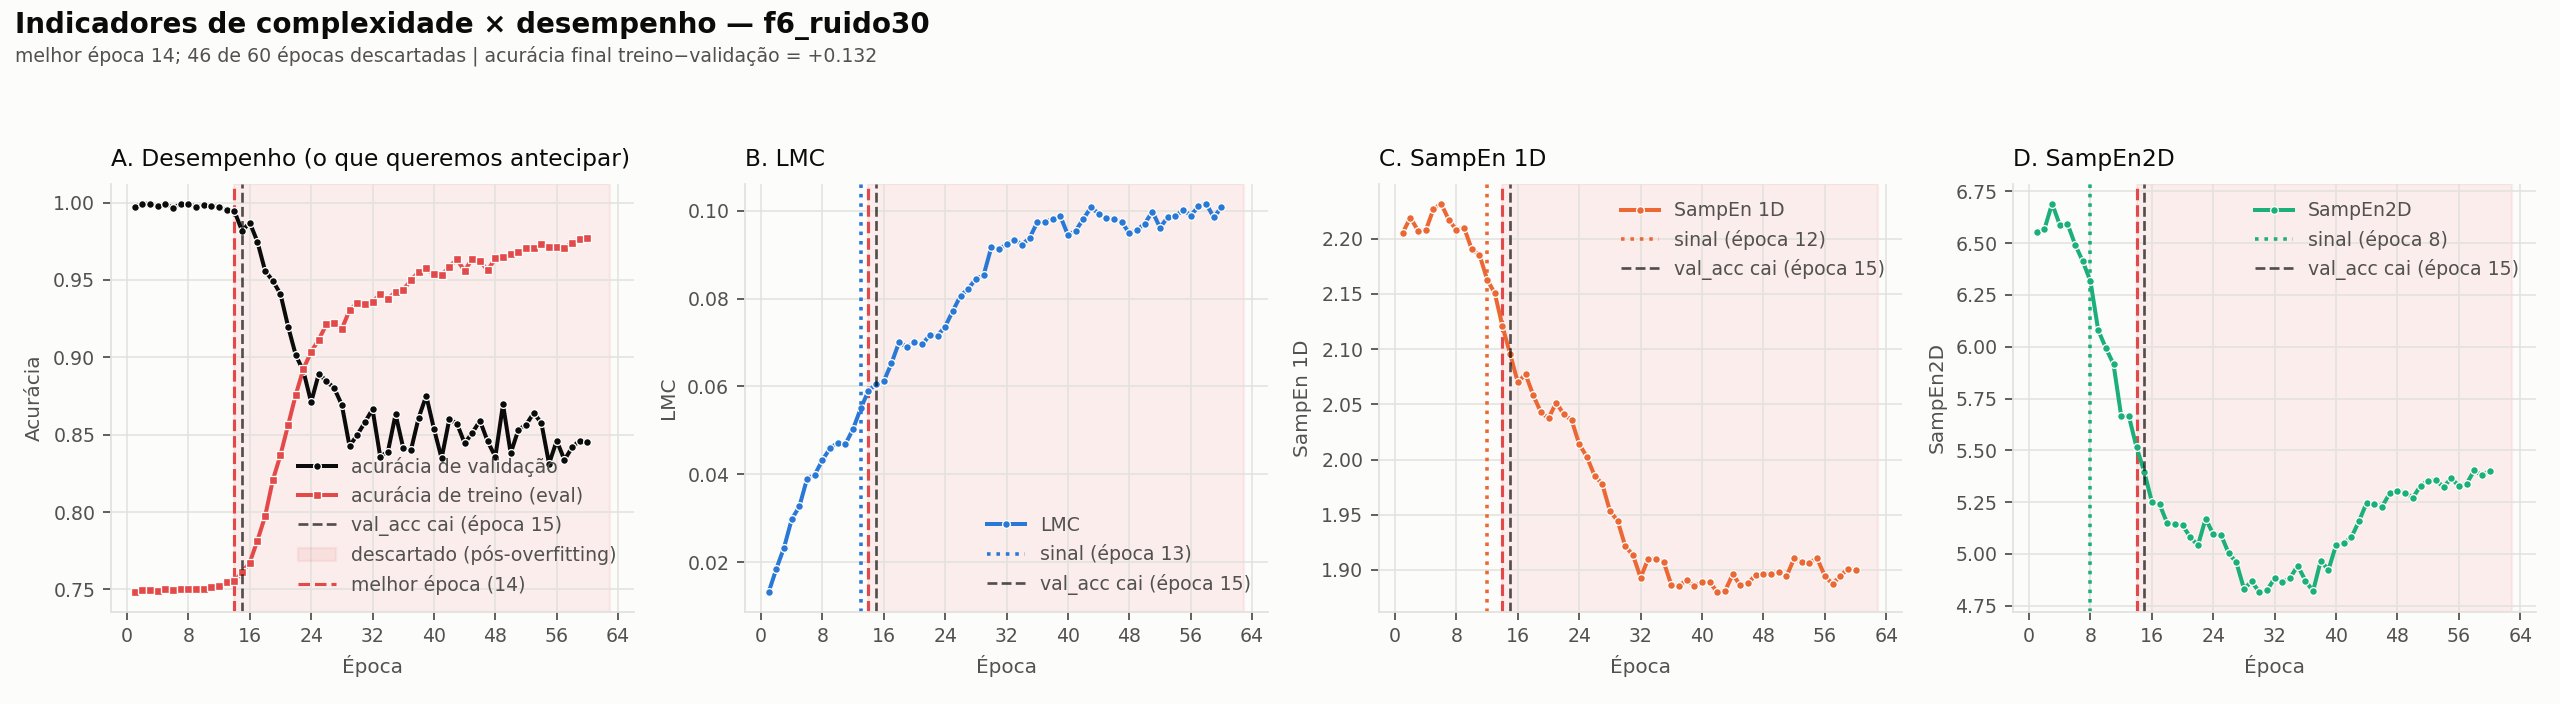
\includegraphics[width=0.95\textwidth]{figuras/indicadores_f6_ruido30.png}
    \caption{Trajetória dos três indicadores e da validação em execução com
    corrupção de \SI{30}{\percent} dos rótulos. A região sombreada corresponde
    às épocas posteriores ao início do \emph{overfitting}, excluídas das
    conclusões.}
    \label{fig:indicadores}
    \fonte{Elaborado pelo autor.}
\end{figure}

\section{Efeito do Nível de Corrupção}
\label{sec:R-niveis}

Variou-se a fração de rótulos corrompidos em \SI{15}{\percent},
\SI{30}{\percent} e \SI{50}{\percent}, com três sementes por nível. O resultado
é instrutivo e não era o esperado.

A época em que o monitor emite o alerta é praticamente invariante ao nível de
corrupção --- médias de \num{10,0}, \num{9,3} e \num{10,0} épocas para os três
níveis, sem diferença estatisticamente detectável
($F = \num{1,00}$; $p = \num{0,42}$). O que se move é a âncora, isto é, o momento
em que a degradação se torna visível na validação, que chega progressivamente
mais cedo com mais corrupção ($F = \num{30,2}$; $p = \num{0,0007}$).

A consequência prática é que a antecedência encolhe à medida que a corrupção
aumenta: aproximadamente \num{7,7} épocas a \SI{15}{\percent}, \num{5,3} a
\SI{30}{\percent} e \num{3,0} a \SI{50}{\percent}. A leitura que se propõe é
que o indicador marca o \emph{início} da memorização, cujo momento depende pouco
da quantidade de rótulos errados, enquanto a validação mede o \emph{sintoma},
que se manifesta tanto mais cedo quanto maior a corrupção. Trata-se de
interpretação plausível, ainda não demonstrada, e que o trabalho pretende
investigar.

\section{Generalização entre Arquiteturas: um Limite Identificado}
\label{sec:R-arquitetura}

O experimento foi repetido com DenseNet-121, em três execuções com corrupção e
três controles. Os resultados são parcialmente favoráveis e devem ser
reportados com precisão.

A antecedência é preservada e de fato ampliada: a SampEn2D inflete \num{20},
\num{21} e \num{17} épocas antes da âncora nas três execuções. Contudo, o poder
de discriminação por amplitude \textbf{cai substancialmente}: a razão entre
execuções com corrupção e controles é de \num{2,8} vezes, contra \num{5,71} na
ResNet-18, e as demais medidas deixam de discriminar (\num{1,3} para a
SampEn 1D e \num{1,2} para a LMC). Com três execuções por grupo, não há poder
estatístico para afirmar significância.

A conclusão honesta é que o achado central foi verificado em uma segunda
arquitetura quanto à antecedência, mas não quanto à magnitude do contraste. Se
isso decorre do tamanho da camada densa, da dinâmica de otimização própria da
DenseNet ou simplesmente do número reduzido de execuções, é questão em aberto e
consta entre os objetivos específicos deste projeto.

\section{Escolha da Âncora}
\label{sec:R-ancora}

Um resultado metodológico merece registro. A primeira versão do monitor ancorava
o diagnóstico na perda de validação. Nessa configuração, o monitor acusava
\emph{overfitting} em dez de dez execuções, incluindo todos os controles,
sinalizando o estado em cerca de metade das épocas mesmo quando não havia
corrupção alguma. A causa é que o MedNIST satura muito cedo, e a perda de
validação começa a subir logo após a primeira época mesmo em treinamentos
saudáveis.

Reancorando o diagnóstico na acurácia de validação, o comportamento tornou-se
o esperado: oito de oito execuções com corrupção sinalizadas, nenhum falso
positivo entre os oito controles. O episódio ilustra que a definição
operacional de \emph{overfitting} não é detalhe de implementação, mas condição
de validade do resultado.

\section{Limitações dos Resultados Atuais}
\label{sec:R-limitacoes}

\begin{enumerate}
    \item Os experimentos restringem-se a um único repositório de imagens, que
          é reconhecidamente fácil e satura rapidamente. A extensão a
          repositórios mais difíceis é necessária.
    \item A memorização é induzida artificialmente. Resta demonstrar que o
          indicador se comporta do mesmo modo diante de \emph{overfitting}
          espontâneo, por escassez de dados e não por corrupção de rótulos.
    \item O contraste em DenseNet-121 é fraco e baseado em três execuções por
          grupo.
    \item Os limiares do monitor foram calibrados em um subconjunto das
          execuções e verificados nas demais; ainda assim, a possibilidade de
          ajuste excessivo do critério aos próprios dados exige validação em
          condições inteiramente novas.
\end{enumerate}


\postextual
\bibliography{referencias}

\end{document}
